\subsection{Сдвинутая прямоугольная функция}
Рассмотрим прямоугольную функция из первого задания (см. формулу~\eqref{eq:rectangle_function}). Примем $a = 1$, $b = 0.5$. 
Рассмотрим \textit{сдвинутую функцию} $g(t) = f(t + c)$

\subsubsection{Графики исходных функции}
Графики данной функции при различных значениях $c$ представлены на рисунках \ref{fig:moved_rectangle_1}, \ref{fig:moved_rectangle_2} и \ref{fig:moved_rectangle_3}.

\begin{figure}[ht!]
    \centering
    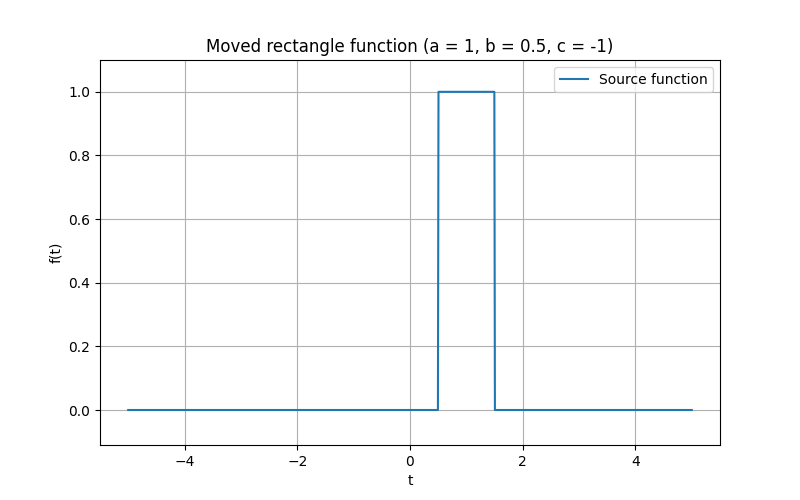
\includegraphics[width=\textwidth]{media/moved_rectangle_1.png}
    \caption{График функции $g(t)$ при $c = -1$}
    \label{fig:moved_rectangle_1}
\end{figure}

\begin{figure}[ht!]
    \centering
    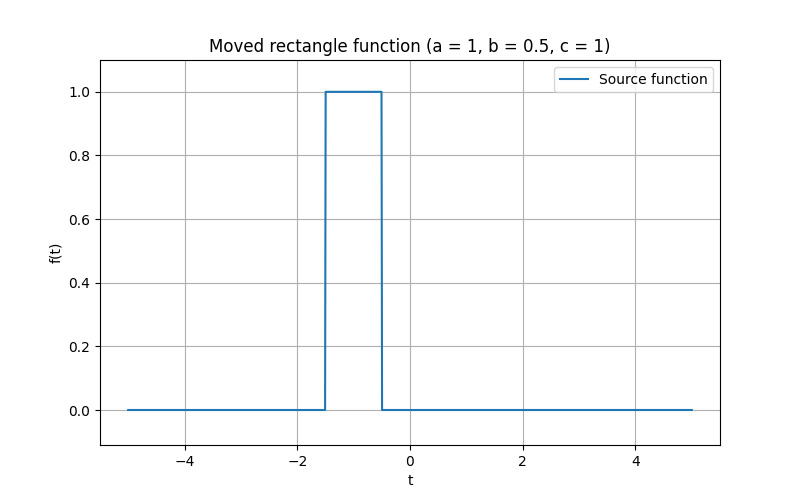
\includegraphics[width=\textwidth]{media/moved_rectangle_2.png}
    \caption{График функции $g(t)$ при $c = 1$}
    \label{fig:moved_rectangle_2}
\end{figure}

\begin{figure}[ht!]
    \centering
    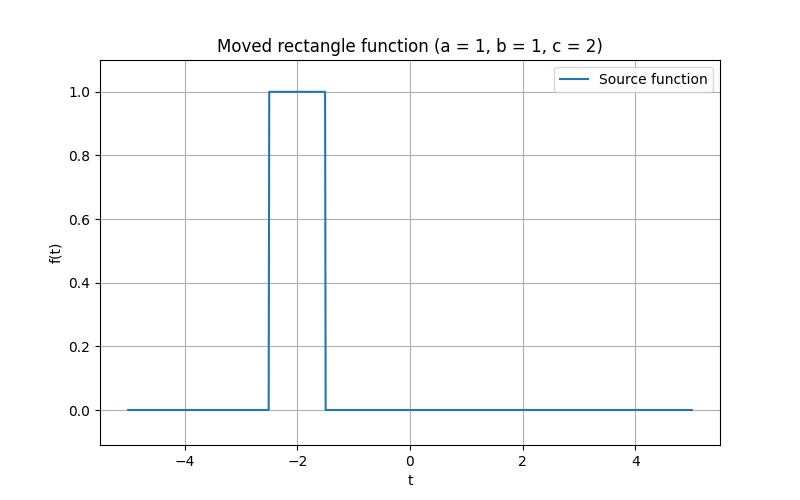
\includegraphics[width=\textwidth]{media/moved_rectangle_3.png}
    \caption{График функции $g(t)$ при $c = 2$}
    \label{fig:moved_rectangle_3}
\end{figure}
\FloatBarrier

\subsubsection{Нахождение образа функции}

Согласно формуле \eqref{eq:image_from_function}, Фурье образ функции $g(t)$ задается следующим выражением:
\begin{multline}
    \hat{g}(\omega) = \frac{1}{\sqrt{2\pi}} \int_{-\infty}^{\infty} g(t) e^{-i\omega t} dt = \frac{1}{\sqrt{2\pi}} \int_{-\infty}^{\infty} f(t + c) e^{-i\omega t} dt = \frac{1}{\sqrt{2\pi}} \int_{-\infty}^{\infty} f(t) e^{-i\omega (t - c)} dt = \\
    \frac{1}{\sqrt{2\pi}} \int_{-b}^{b} a e^{-i\omega (t - c)} d(t - c) = \frac{a}{-\omega i\sqrt{2\pi}} e^{-i\omega (t - c)} \Biggr|_{-b}^{b} = \frac{a(e^{i\omega (b + c)} - e^{-i\omega (b - c)})}{\omega i \sqrt{2 \pi}} = \frac{a e^{i\omega c} (e^{i\omega b} - e^{-i\omega b})}{\omega i \sqrt{2\pi}} =\\
    \frac{2ae^{i\omega c} \sin{\omega b}}{\omega \sqrt{2\pi}} = \frac{2abe^{i\omega c}}{\sqrt{2\pi}}\sinc{\omega b}
    \label{eq:moved_rectangle_image}
\end{multline}

Заметим, что относительно прошлого образа функции (см. формулу~\eqref{eq:rectangle_image}) добавился множитель $e^{i\omega c}$. Он отвечает за \textit{поворот} образа в комплексной плоскости. Таким образом, образ сдвинутой функции является комплексным. 

\subsubsection{Графики образов функций}
Графики образов функции при различных значениях $c$ представлены на рисунках \ref{fig:moved_rectangle_1_image}, \ref{fig:moved_rectangle_2_image} и \ref{fig:moved_rectangle_3_image}.

\begin{figure}[ht!]
    \centering
    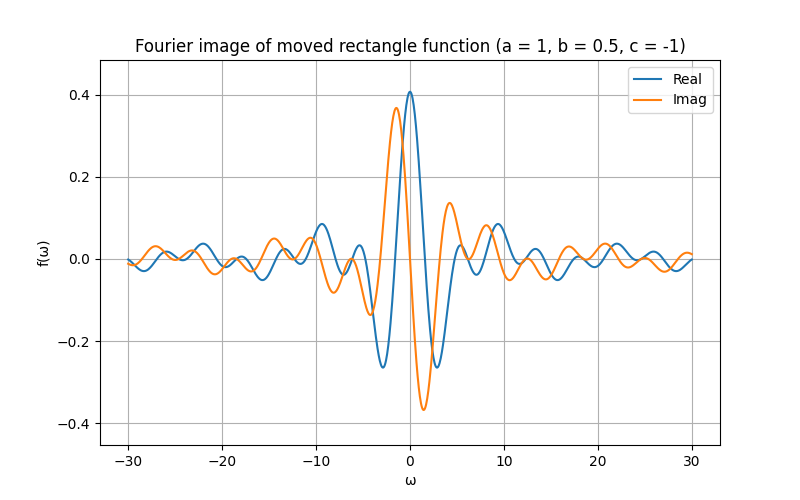
\includegraphics[width=\textwidth]{media/moved_rectangle_1_image.png}
    \caption{График образа функции $g(t)$ при $c = -1$}
    \label{fig:moved_rectangle_1_image}
\end{figure}

\begin{figure}[ht!]
    \centering
    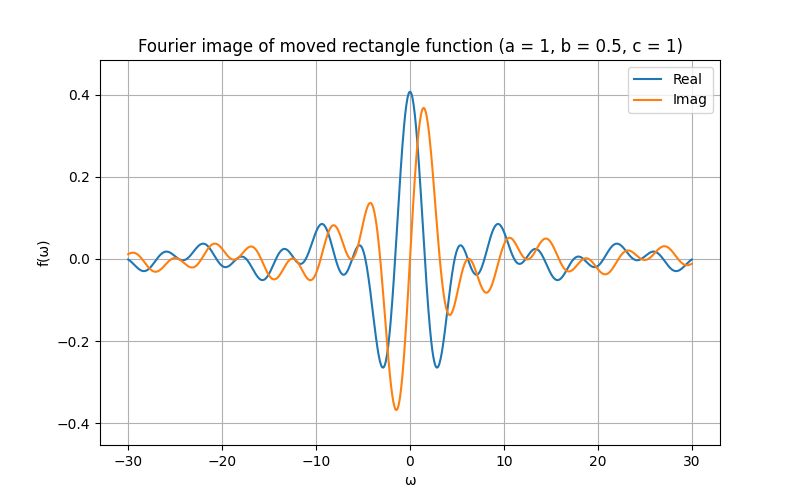
\includegraphics[width=\textwidth]{media/moved_rectangle_2_image.png}
    \caption{График образа функции $g(t)$ при $c = 1$}
    \label{fig:moved_rectangle_2_image}
\end{figure}

\begin{figure}[ht!]
    \centering
    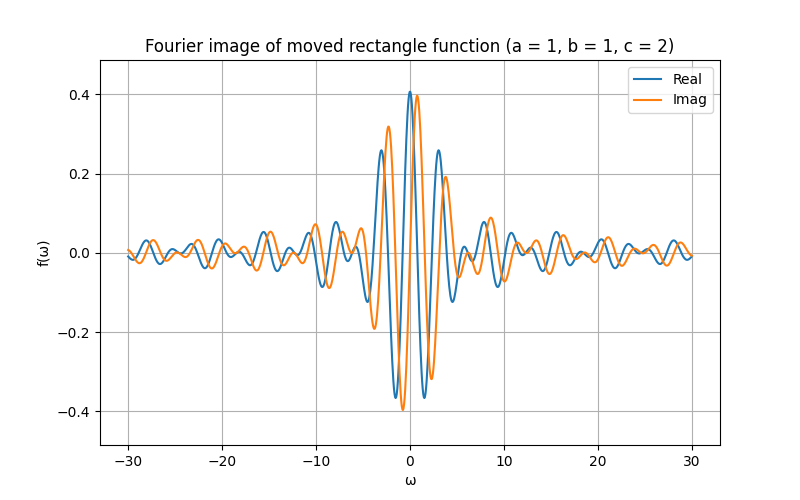
\includegraphics[width=\textwidth]{media/moved_rectangle_3_image.png}
    \caption{График образа функции $g(t)$ при $c = 2$}
    \label{fig:moved_rectangle_3_image}
\end{figure}

Кроме того, рассмотрим графики модуля образа функции на рисунках \ref{fig:moved_rectangle_1_image_abs}, \ref{fig:moved_rectangle_2_image_abs} и \ref{fig:moved_rectangle_3_image_abs}.

\begin{figure}[ht!]
    \centering
    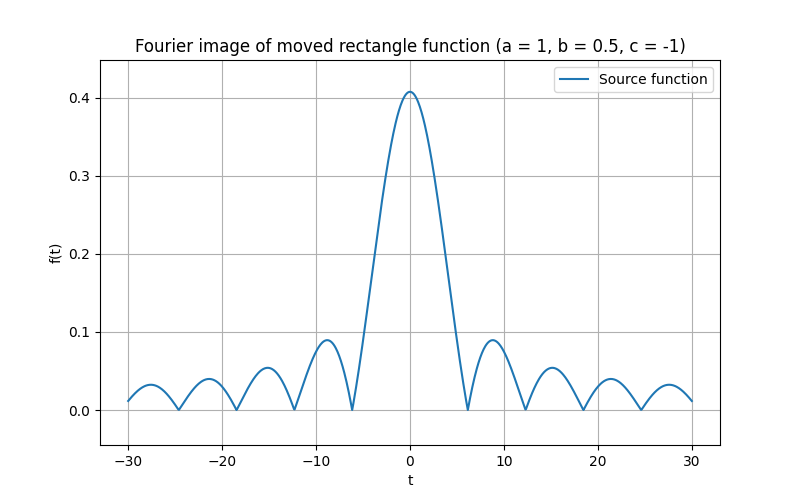
\includegraphics[width=\textwidth]{media/moved_rectangle_1_image_abs.png}
    \caption{График модуля образа функции $g(t)$ при $c = -1$}
    \label{fig:moved_rectangle_1_image_abs}
\end{figure}

\begin{figure}[ht!]
    \centering
    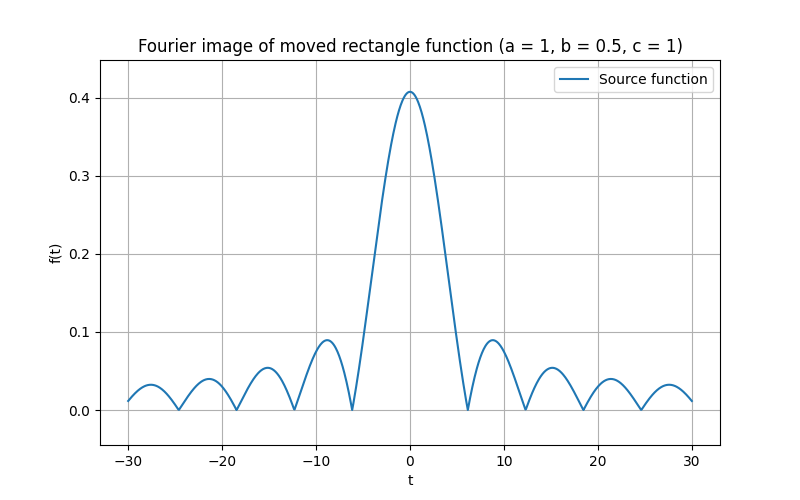
\includegraphics[width=\textwidth]{media/moved_rectangle_2_image_abs.png}
    \caption{График модуля образа функции $g(t)$ при $c = 1$}
    \label{fig:moved_rectangle_2_image_abs}
\end{figure}

\begin{figure}[ht!]
    \centering
    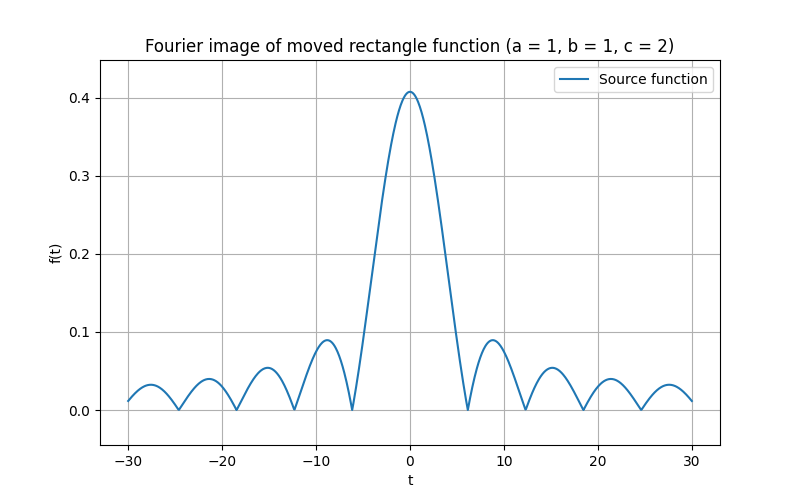
\includegraphics[width=\textwidth]{media/moved_rectangle_3_image_abs.png}
    \caption{График модуля образа функции $g(t)$ при $c = 2$}
    \label{fig:moved_rectangle_3_image_abs}
\end{figure}

Видим, что графики модуля образа функции не отличаются в зависимости от значения $c$. Это связано с тем, что модуль комплексного числа не зависит от его аргумента.

\FloatBarrier

\subsubsection{Проверка равенства Парсеваля}
Проверим равенство Парсеваля (см. формулу~\eqref{eq:parseval_indentity}). Для этого воспользуемся функцией \texttt{parseval\_check}. 

\begin{table}[ht!]
    \centering
    \begin{tabular}{|c|c|}
        \hline
        $\displaystyle\int_{-100}^{100}{|g(t)|^2}$ & $\displaystyle\int_{-100}^{100}{|\hat{g_1}(\omega)|^2}$ \\
        \hline
        1.0010 & 0.9946 \\
        \hline
    \end{tabular}
    \caption{Результаты проверки равенства Парсеваля для сдвинутой прямоугольной функции $g(t)$ при $a = 1$, $b = 0.5, c = -1$}
    \label{tab:moved_rectangle_1_parseval_check}
\end{table}

\begin{table}[ht!]
    \centering
    \begin{tabular}{|c|c|}
        \hline
        $\displaystyle\int_{-100}^{100}{|g(t)|^2}$ & $\displaystyle\int_{-100}^{100}{|\hat{g_2}(\omega)|^2}$ \\
        \hline
        1.00100 & 0.9946 \\
        \hline
    \end{tabular}
    \caption{Результаты проверки равенства Парсеваля для сдвинутой прямоугольной функции $g(t)$ при $a = 1$, $b = 0.5, c = 1$}
    \label{tab:moved_rectangle_2_parseval_check}
\end{table}

\begin{table}[ht!]
    \centering
    \begin{tabular}{|c|c|}
        \hline
        $\displaystyle\int_{-100}^{100}{|g(t)|^2}$ & $\displaystyle\int_{-100}^{100}{|\hat{g_3}(\omega)|^2}$ \\
        \hline
        0.5005 & 0.49417 \\
        \hline
    \end{tabular}
    \caption{Результаты проверки равенства Парсеваля для сдвинутой прямоугольной функции $g(t)$ при $a = 1$, $b = 0.5, c = 2$}
    \label{tab:moved_rectangle_3_parseval_check}
\end{table}
Видим, что полученные значения практически равны. Разница, как и в случае с \textit{не сдвинутыми} функциями обусловлена интегрированием не по всей числовой прямой, а лишь по ее части.

\subsubsection{Анализ результатов}
Видим, что при увеличении значения $c$ график исходной функции, очевидно, сдвигается, а график ее образа \textit{сжимается}, при этом амплитуда остается неизменной. 